\documentclass[
	%a4paper, % Use A4 paper size
	letterpaper, % Use US letter paper size
]{jdf}

\usepackage{float}
\usepackage{minted}

\addbibresource{references.bib}

\author{Matt Wong}
\email{mwong82@gatech.edu}
\title{Homework 1 | CS-6291: Embedded Software}

\begin{document}
%\lsstyle

\maketitle

\setlength{\parskip}{\baselineskip}%
\section{Question 1}

\subsection{Question 1.1}
\textit{What is the speed-up of the above program for a VLIW machine with one ALU unit and unlimited other functional units?}

The speed-up is mathematically defined as the total time to execute sequentially / ((time required by parallel parts/number of parallel resources) + time required by sequential parts.

In the case that the functional units aside from the ALU are unlimited, then the time to execute the parallel parts would be 0.
Therefore, with 1 ALU unit and the program containing 45 percent ALU ops, the function then becomes:
\begin{minted}{python}
1/(0)+(.45/1)
\end{minted}{python}

As a result, the speed-up is 2.22.

\subsection{Question 1.2}
\textit{What is the speed-up for a VLIW machine with two memory units, two integer units, three floating-point units, and one branch unit?}

The speed-up for a VLIW machine with the previously described units could be represented with the following function:

\begin{minted}{python}
1/((.14/2)+(.45/2)+(.3/1)+(.11/3))
\end{minted}{python}

This comes out to a speed-up of 1.58.

\section{Question 2}

\subsection{Question 2.1}
\textit{Can operations A and B be scheduled in the same cycle? If not, please note the register and type of dependency.}

Operations A and B cannot be scheduled in the same cycle. This is because there is a dependency of type RAW with reading from register r5 in operation B after writing to r5 in operation A. However, this can be resolved developing a mechanism to block an read instruction before the write is complete, and the hardware will have to keep track of this.

\subsection{Question 2.2}
\textit{Can operations B and C be scheduled in the same cycle? If not, please note the register and type of dependency.}

Yes, they can. There are no dependencies between these two operations.

\subsection{Question 2.3}
\textit{Can operation E be scheduled ahead of operation D? If not, please note the register and type of dependency.}

Operation E cannot be schedule ahead of operation D, because there is a dependency of RAW between E and D. Specifically, E needs to read from register r1, and operation D writes a value to r1. Therefore, E cannot be scheduled before D. However, this can be resolved by developing a mechanism to block an read instruction before the write is complete, and the hardware will have to keep track of this.

\subsection{Question 2.4}
\textit{Can operation F be scheduled ahead of operation E? If not, please note the register and type of dependency.}

F cannot be scheduled ahead of E, and the reason is because there is a dependency of type WAW. Both F and E write to register r5, and if F was scheduled ahead of E, it is likely that the first write will be the final value kept in r5 at program completion, which would cause an undesired behavior relative to the expectation.

\section{Question 3}

\subsection{Question 3.1}
\textit{Which VEX operations are scheduled together as the second VLIW instruction?}

My answer to this is that only VEX operation C is the only operation scheduled as the second VLIW instruction. The rationale for this is because operations in the same instruction cannot have any dependencies between them. This means any dependency of type RAW, WAW, or WAR. Additionally, operations should be scheduled as soon as possible. With no limitations on resources and infinite operations per instruction, we can at most schedule A and B in the first instruction, as no dependencies between them exist. However, we cannot schedule C in the first instruction, because both operation A and C write to register r1. Therefore, we can schedule operation C in the second cycle, however the remaining operations all read or write from/to register r1, so C is the only operation that can exist in the second instruction.
\begin{minted}{python}
q3_1 = ["C"]
\end{minted}{python}
\subsection{Question 3.2}
\textit{Assume each VLIW instruction consumes 2 cycles. Calculate the average IPC, which is a ratio of the total number of operations executed to the total number of cycles needed.}

Under this optimized instruction set, we have 6 vex operations contained in 5 instructions, with each instruction taking 2 cycles each. This results in a IPC (operations per cycle) of 6 operations / 10 cycles, or 0.6.

\begin{minted}{python}
q3_2 = 0.60
\end{minted}{python}

\section{Question 4}
\subsection{Question 4.1}
\textit{What is the CPI for sequential execution of the code?}

The CPI for sequential execution of the code can be represented as the sum of the cycles(or latencies)/total operations.
\begin{minted}{python}
3+5+4+3+3+3/6 = 21/6 
\end{minted}{python}

This results in a CPI of 3.50.

\subsection{Question 4.2}
\textit{Assume register renaming is now added to the processor. Does it allow you to improve CPI by scheduling instructions sooner than without this technique?}

If register renaming is supported, CPI can be improved to 2.33 with the following schedule:

\begin{minted}{python}
q4_2 = 2.33
q4_2schedule = ["sub $r2 = $r1, $r2",
                "",
                "",
                "stw 8[$r4] = $r2",
                "",
                "",
                "",
                "",
                "ldw $r6 = 8[$r4]",
                "mpy $r3 = $r7, $r7",
                "sub $r8 = $r5, $r1",
                "mpy $r9 = $r5, $r1",
                "",
                ""
                ]
\end{minted}{python}

There is a false data dependency that exists for instruction D, which writes to register r4, but depends on the read from instruction C's r4 read. If register renaming is allowed, instruction D's output can be stored in a new register, r3, instead. Then instead of waiting for the full 4-cycle latency from instruction C, it can be issued immediately in the next cycle. Similarly, instruction E has a dependency of type WAR for r7, and with register renaming can execute immediately if the output register is changed to r8. Lastly, instruction F can write back to a new register, r9, so that it can execute in the cycle after E by avoiding the WAR dependency. We cannot improve instruction A-C latencies with register renaming, as these are true dependencies.

\section{Question 5}
\subsection{Question 5.1}
\textit{What is the CPI for sequential execution of the code with no data speculation}

The CPI for sequential execution with no data speculation would be calculated the same way as the previous example, by summing the latencies and dividing by the number of instructions:

\begin{minted}{python}
5+7+5+7/4 = 24/4
\end{minted}{python}

The CPI is 6.0.

\subsection{Question 5.2}
\textit{Create a new schedule to maximize instruction level parallelism (ILP) using instruction scheduling and data speculation, but without register renaming.}
With data speculation, we can schedule instructions before knowing they can be executed correctly. With regard to instructions A, B, and C, we have register offset dependencies, but with data speculation, we can schedule them one after the other as opposed to waiting the full latency of each instruction. However, the exception to this is with instruction D. Instruction D has a true RAW dependency of reading from r2 after C writes into it, so it must wait the full latency of ldw (5) before being scheduled.

\begin{minted}{python}
q5_2_schedule = ["A", "B", "C", "", "","", "", "D", "", "", "", "", "", ""]
\end{minted}{python}

The new CPI is 14 cycles / 4 instructions, which is 3.50.

\section{Question 6}

\subsection{Question 6.1}
\textit{Determine the data dependence graph for the above code}

\begin{figure}[H]
	\centering
	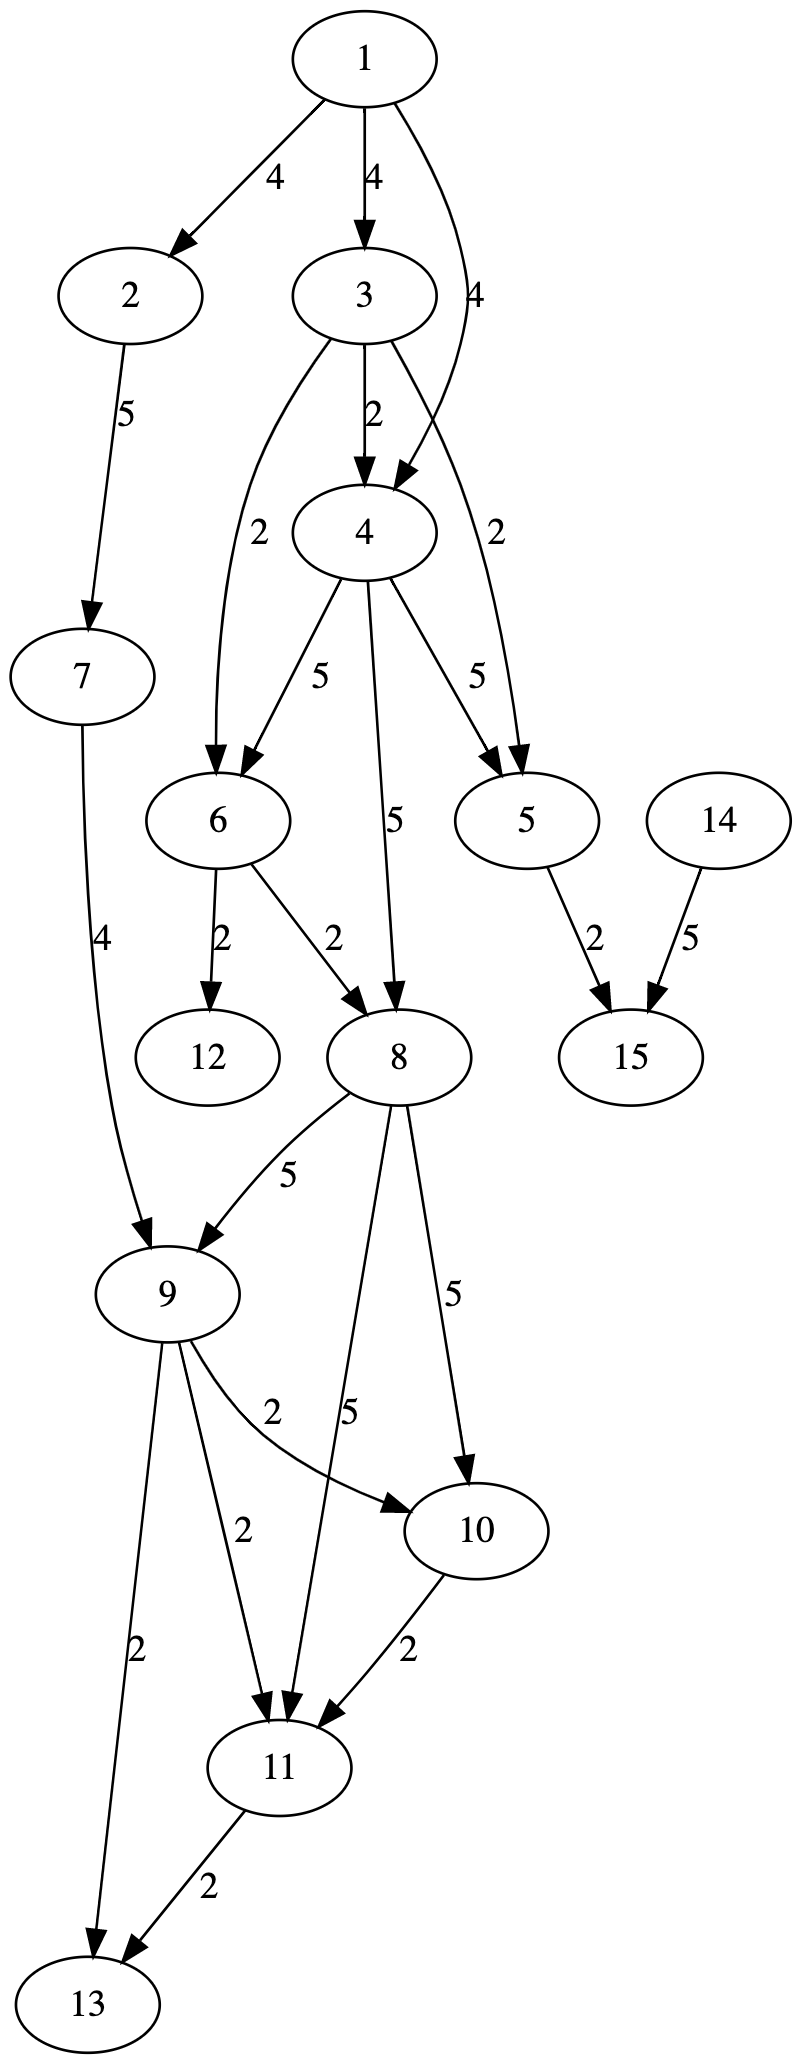
\includegraphics[height=15cm]{Figures/graphviz.png}
	\caption{Dependency graph for question 6's VEX code, including direct, and indirect dependencies.}
	\label{fig:flowchart}
\end{figure}

The graph represented in the Python code, where each entry represented an edge between two nodes on the graph (including grandchild dependencies) was:
\begin{minted}{python}
q6_1 = [
    "1 -> 2",
    "1 -> 3",
    "1 -> 4" 
    "2 -> 7",
    "3 -> 4", 
    "3 -> 5",
    "3 -> 6"
    "4 -> 5",
    "4 -> 6", 
    "4 -> 8", 
    "5 -> 15",
    "6 -> 12",
    "6 -> 8", 
    "7 -> 9", 
    "8 -> 9", 
    "8 -> 10", 
    "8 -> 11", 
    "9 -> 10", 
    "9 -> 11", 
    "9 -> 13",
    "10 -> 11", 
    "11 -> 13", 
    "14 -> 15" 
]
\end{minted}{python}
\subsection{Question 6.2}
\textit{Using the dependence graph and given latencies, find the shortest possible valid instruction schedule. Make your schedule as follows}

With the dependence graph illustrated above, the shortest possible valid instruction schedule could be represented with the following python code, where each entry in the array represents an cycle for a 4-slot machine. The numbers in each slot correspond to each operation executed in that particular VLIW instruction for that cycle.

\begin{minted}{python}
q6_2 = [
        ["", "14", "", "1"],
        ["", "", "", ""],
        ["", "", "", ""],
        ["", "", "", ""],
        ["3", "2", "", ""],
        ["", "", "", ""],
        ["", "4", "", ""],
        ["", "", "", ""],
        ["", "", "", ""],
        ["", "", "", "7"],
        ["", "", "", ""],
        ["6", "8", "", ""],
        ["5", "", "", ""],
        ["12", "", "", ""],
        ["15", "", "", ""],
        ["9", "", "", ""],
        ["10", "", "", ""],
        ["", "", "", ""],
        ["11", "", "", ""],
        ["", "", "", ""],
        ["13", "", "", ""],
        ["", "", "", ""],
        ["", "", "", ""]
        ]
\end{minted}{python}
\subsection{Question 6.3}
\textit{Calculate the number of cycles it takes to execute the VLIW code.}

With the optimized schedule, it takes a total of 23 cycles to execute the program.


\subsection{Question 6.4}
\textit{How many slots do not have an operation scheduled in them? Provide the ratio of empty slots to the total number of slots present in the instruction schedule. Do not simplify the fraction; we want to see you selected the correct number of total slots and empty slots.}

77 / 92 slots for the functional units are unoccupied throughout the execution of the program, if we are saying that "occupied" is constituted as being able to hold a new operation at each cycle. If we are assuming that each slot is actually occupied over multiple cycles due to the latencies associated with a particular instruction, then instruction numbers would be duplicated across cycles, and then less slots would be blank, but I'm illustrating the each slot as holding an instruction only once it is scheduled.

\end{document}
